\documentclass[11pt]{article}
\usepackage{royden-report}
\usepackage[T1]{fontenc}
\usepackage{lmodern}
\usepackage{microtype}
\title{A numerical reference for the spatial Dysthe equation}
\author{Stage one: local reference validation}
\date{16 October 2026}
\newcommand{\ii}{\mathrm{i}}
\newcommand{\normtwo}[1]{\left\lVert #1\right\rVert_{2,L}}
\newcommand{\opD}{\lvert D_\tau\rvert}
\begin{document}
\maketitle
\begin{abstract}
A bounded local campaign tests the existing water-wave reference before
initial-data simulation or operator learning. Analytic controls, independent
residuals, invariant audits, and separate step, grid, and domain comparisons
qualify the stated periodic problem. Matched propagated controls separate
phase and translation drift from deformation. Finite-window persistence
establishes neither soliton discovery nor spectral or nonlinear stability.
\end{abstract}

\section{Equation and discretization}
The verified project is
\begin{quote}\small
\path{/home/matasvai/Documents/Projects/Dysthe}.
\end{quote}
The contract \texttt{water-wave-dysthe-spatial-v1} specifies the complex scaled
free-surface envelope $u(\xi,\tau)$, propagation distance $\xi$, and retarded
time $\tau$:
\begin{equation}\label{eq:dysthe}
 u_\xi=-\ii u_{\tau\tau}-\ii\lvert u\rvert^2u
 -\epsilon\left(8\lvert u\rvert^2u_\tau
       +2u^2\overline{u_\tau}
       +2\ii u\opD(\lvert u\rvert^2)\right).
\end{equation}
This is equation (1.3) of Fedele and Dutykh \cite{fedele2012}, with
$(a,h,c,e,f)=(1,1,8,2,2)$. The source normalization is $B=\epsilon u$,
$\tau=\epsilon(2x-t)$, $\xi=\epsilon^2x$, and $\epsilon=k_0a$ in
dimensionless carrier coordinates. The $\epsilon=0$ NLS control is a
mathematical limit; the coordinate transformation degenerates there.
Complex128 arrays have axes $[\xi,\tau]$, not two horizontal directions.

The domain $I_L=[-L/2,L/2)$ is periodic, with
$\tau_j=-L/2+jL/N$, $0\leq j<N$. No absorbing layer is used.
For Fourier kernel $e^{-\ii k\tau}$ and $k_m=2\pi m/L$,
$\partial_\tau$ has symbol $\ii k_m$ and $\opD$ has symbol
$\lvert k_m\rvert$, including a zero mean mode. Thus
$\opD=\mathcal H\partial_\tau$ with Hilbert symbol
$-\ii\operatorname{sign}(k_m)$.

Let $P_N$ retain the strict band $\lvert m\rvert<N/4$, let $\mathcal F$
be the full RHS of \eqref{eq:dysthe}, and let
$\mathcal L=-\ii\partial_{\tau\tau}$. The computed Galerkin system is
\begin{equation}\label{eq:galerkin}
 u_\xi=\mathcal L u+P_N(\mathcal F(u)-\mathcal L u),\qquad u=P_Nu.
\end{equation}
This band resolves retained cubic products without aliasing. Lawson
integrating-factor RK4 applies $\exp(\ii k_m^2\Delta\xi)$ exactly and
advances the transformed nonlinear equation with classical RK4.
Petviashvili-type profile construction restricts conjugate reflection;
propagation imposes no such symmetry. Iteration convergence does not
establish stability or enumerate all branches.

\section{Controls and diagnostics}
Use $\normtwo{f}^2=\int_{I_L}|f|^2\,\rad\tau$, discretized by
$(L/N)\sum_j|f_j|^2$. Linear multiplier tests and explicit Fourier
convolution of a nonconstant complex multimode field check signs,
conjugation, and nonzero mean flow. Exact periodic plane waves satisfy
\begin{equation}\label{eq:plane}
 u=Ae^{\ii k\tau-\ii\Omega\xi},\qquad
 \Omega=A^2-k^2+6\epsilon kA^2,\quad kL/(2\pi)\in\ZZ.
\end{equation}
The implementation's traveling convention is tested at $\epsilon=0$ by
\begin{equation}\label{eq:nls}
\begin{aligned}
 u(\xi,\tau)&=e^{-\ii\mu\xi}F(\tau-s\xi),\\
 F(\tau)&=\sqrt{2\nu}\operatorname{sech}(\sqrt\nu\,\tau)e^{-\ii s\tau/2},
 \qquad \nu=\mu-s^2/4>0.
\end{aligned}
\end{equation}
This whole-line solution requires negligible periodic-window error.
Nonzero $s$ tests translation and phase; a moving Dysthe profile supplies
an additional control.

For a profile $F$, let $T=-\ii\mu F-sF_\tau\ne0$. Fourfold Fourier
interpolation resolves its full cubic RHS and gives independent residuals
\begin{equation}\label{eq:residual}
\begin{aligned}
 r_{\rm full}&=\frac{\normtwo{\mathcal F(F)-T}}{\normtwo{T}},&
 r_{\rm ret}&=\frac{\normtwo{P_N[\mathcal F(F)-T]}}{\normtwo{T}},\\
 r_{\rm disc}&=\frac{\normtwo{(1-P_N)\mathcal F(F)}}{\normtwo{T}}.
\end{aligned}
\end{equation}
These qualify the trigonometric interpolant, not whole-line existence or
accumulated propagation error. Arbitrary-field discarded-RHS diagnostics
instead normalize by $\normtwo{\mathcal F(u)}$ and record that choice.

With $\rho=|u|^2$ and $J=\operatorname{Im}(u_\tau\overline u)$, monitor
\begin{align}
 \mathcal A&=\int_{I_L}\rho\,\rad\tau,\label{eq:action}\\
 \mathcal M&=\int_{I_L}(2J-2\epsilon\rho^2)\,\rad\tau,\label{eq:momentum}\\
 \mathcal E&=\int_{I_L}\left(|u_\tau|^2-\tfrac12\rho^2
 +\tfrac{10}{3}\epsilon^2\rho^3-5\epsilon\rho J
 -\epsilon\rho\opD\rho\right)\,\rad\tau.\label{eq:energy}
\end{align}
These are continuum functionals \cite{fedele2012}; $u$ is noncanonical,
and no periodic canonical gauge is imposed. Quadrature on $2N$ interpolated
points resolves the degree-six density: $6K<2N$ for retained cutoff
$K<N/4$. An independent directional-derivative audit uses both full and
Galerkin RHSs. Projection can change energy/momentum conservation; RK4
can change action. Absolute drift is retained, with relative drift omitted
near zero. Conservation alone does not establish accuracy.

For perturbed field $w$ and its matched propagated control $v$, fit only
translation $a$ and constant phase $\theta$:
\begin{equation}\label{eq:fit}
 D_{\rm shape}=\min_{a,\theta}
 \frac{\normtwo{w-e^{\ii\theta}v(\cdot-a)}}{\normtwo{v}},\qquad
 q=e^{-\ii\theta}w(\cdot+a)-v.
\end{equation}
All discrete translations are searched, followed by correlation refinement
and polishing; continuous global optimality is not proved. Regression
controls test roundoff symmetry recovery and preservation of amplitude
changes. Raw error, periodic translation, and principal-valued phase remain
separate. Comparing signed fields $q$ between refinements retains radiation
and deformation that differences of scalar norms would miss.

Step comparisons fix $N,L$; grid comparisons fix $L,\Delta\xi$; domain
comparisons preserve $L/N,\Delta\xi$ and recompute profiles. Common-window
errors and larger-domain exterior norms are reported separately.
Periodicity affects mean flow even with negligible boundary amplitude.
Far-field group speed $-2k$ and folding exterior radiation into a smaller
period diagnose wrapping; neither provides a nonlinear error bound.
Boundary and spectral-edge action are supporting diagnostics. Weak-amplitude
and narrowband screens are design choices, not universal physical bounds.

\section{Measured results and decision}

% Generated by stage1/plot_controls.py; do not edit numerical values here.
% analytic-checks.json SHA-256: 052e4635061b7596c9093604ea3413d86902094092e41997acb327e9e1dba4c4
\subsection{Analytic controls and original-profile audit}
The existing test suite passes 40 tests and 34 subtests
(\path{../results/tests.log}),
including the explicit multimode convolution check with nonzero mean flow.
For plane waves $A=0.6$, $k=0,\pm3$, the largest RHS error is
$1.43\times10^{-12}$ and the largest propagated complex error at
$\xi=2$ is $1.45\times10^{-13}$.
The moving NLS control at $N=2048$, $L=80$, $\mu=2$, $s=1$ has the errors
in Table~\ref{tab:nls}. Successive observed orders approach four
(Figure~\ref{fig:controls}a). Here $p=\log(e_{\rm coarse}/e_{\rm fine})/
\log(h_{\rm coarse}/h_{\rm fine})$; these are exact-solution errors, not
estimates inferred from conservation.

\begin{table}[htbp]
\centering
\caption{Moving NLS complex relative L2 error at $\xi=2$. The ratio compares
with the preceding coarser step.}\label{tab:nls}
\begin{tabular}{rrrr}
\toprule
$\Delta\xi$ & Error & Ratio & Order $p$ \\
\midrule
0.04 & $3.79\times10^{-4}$ & --- & --- \\
0.02 & $2.56\times10^{-5}$ & 14.767 & 3.884 \\
0.01 & $1.65\times10^{-6}$ & 15.548 & 3.959 \\
0.005 & $1.04\times10^{-7}$ & 15.823 & 3.984 \\
\bottomrule
\end{tabular}
\end{table}

A recomputed moving Dysthe profile ($\epsilon=0.025$, $\mu=2$, $s=1$,
$N=4096$, $L=160$) has full residual
$2.06\times10^{-11}$.
At $\xi=2$ and $\Delta\xi=0.000625$,
its raw complex error against the declared traveling solution is
$9.66\times10^{-12}$.

On two independent multimode test fields, full-RHS directional rates of
$\mathcal A,\mathcal M,\mathcal E$ are at most $3.24\times10^{-12}$
in absolute value per unit $\xi$, while the near-cutoff Galerkin energy
rate is $5.92\times10^{-5}$. This explicitly exposes a
projection contribution to invariant drift.


All 28 original stored profiles were independently re-audited on their
original $N=2048$, $L=160$ grid (Figure~\ref{fig:controls}b).
Although every retained residual is at most $4.36\times10^{-11}$,
22 full periodic residuals exceed the current $10^{-8}$ gate.
The largest is $6.12\times10^{-3}$ at
$(\epsilon,\mu,s)=(0.15,3,0)$;
16 profiles also exceed the $\epsilon\max|F|\leq0.1$ design screen.
These results require requalification or finer profile grids; they do not
establish physical instability or nonexistence. The CSV audit retains the
per-profile hashes, residual components, and separate gate decisions.

\begin{figure}[htbp]
\centering
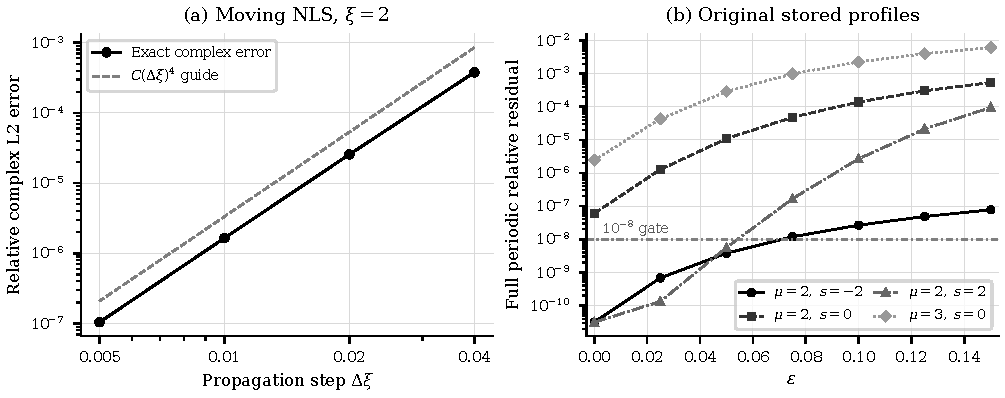
\includegraphics[width=\linewidth]{figures/controls.pdf}
\caption{Analytic propagation control and original-profile full-equation audit.
The dashed fourth-order guide is scaled for visibility. The profile gate
uses the full residual of \eqref{eq:residual}, not the iteration residual.}
\label{fig:controls}
\end{figure}


\subsection{Separate propagation-step and grid checks}

The reused October runs contain 28 trajectories, distinct from the 28 stored branch profiles. Their core and campaign hashes still match the current propagator. Ten new full-horizon trajectories and a two-trajectory short benchmark were run locally; no scheduler or paid compute was used. All new Dysthe cases use $\epsilon=.025$, $\mu=2$, $s=0$, and $0\leq\xi\leq20$. The odd perturbation is $F[1+10^{-3}(\tau/2)e^{-(\tau/2)^2}]$, projected before propagation.

The step table compares successive runs at fixed $L=160$, $N=4096$. Its numbers are maxima over integer samples of $\xi$, normalized by the fine profile norm.

\begin{center}
\small
\begin{tabular}{lrrr}
\toprule
$\Delta\xi$ pair & Control field & Odd field & Signed shape \\
\midrule
0.005 / 0.0025 & $5.96\times10^{-6}$ & $5.96\times10^{-6}$ & $2.08\times10^{-10}$ \\
0.0025 / 0.00125 & $2.96\times10^{-7}$ & $2.96\times10^{-7}$ & $7.90\times10^{-12}$ \\
0.00125 / 0.000625 & $1.66\times10^{-8}$ & $1.66\times10^{-8}$ & $4.65\times10^{-13}$ \\
\bottomrule
\end{tabular}
\end{center}


The final-control observed orders are 4.335 and 4.154. At the smallest historical pair, the maximum raw-field difference is $1.66\times10^{-8}$. Conservation cannot expose this phase-sensitive error by itself.

\begin{center}
\small
\begin{tabular}{lrr}
\toprule
Fixed-domain grid pair & Odd field & Signed shape \\
\midrule
$L=160$: $4096/8192$ & $2.45\times10^{-14}$ & $1.51\times10^{-14}$ \\
$L=320$: $8192/16384$ & $2.67\times10^{-13}$ & $2.31\times10^{-14}$ \\
\bottomrule
\end{tabular}
\end{center}


Both grid comparisons fix $\Delta\xi=.000625$; Fourier interpolation puts each pair on the finer grid. Thus enlarging the domain is not being confused with raising the retained physical wavenumber cutoff.

\begin{figure}[htbp]\centering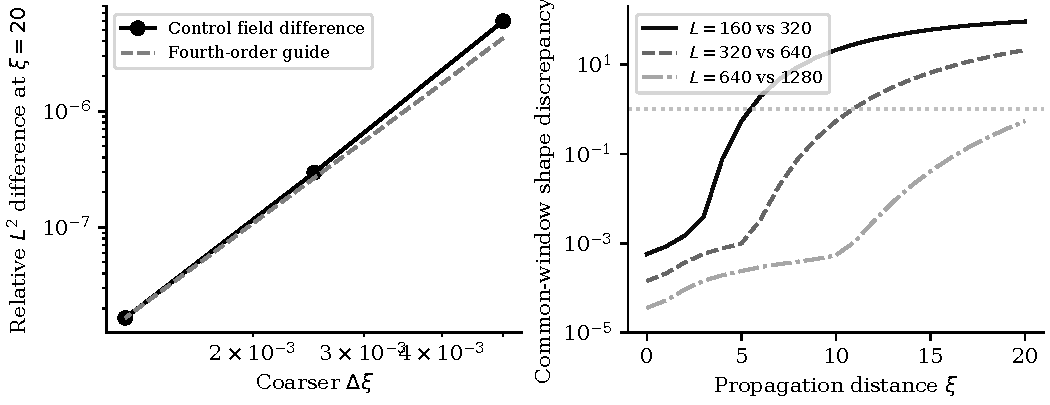
\includegraphics[width=\linewidth]{figures/convergence.pdf}\caption{Step convergence and signed weak-response domain discrepancies. The domain panel uses the fine response norm on the common window; the dotted line is a one-percent comparison target, not a rigorous bound.}\end{figure}

\subsection{Domain sensitivity and the weak odd response}

The domain sequence doubles $L=160,320,640,1280$ at fixed $L/N=160/4096$ and $\Delta\xi=.000625$. Each periodic profile is recomputed. The table gives results at $\xi=20$; shape and core differences are normalized by the fine carrier profile on the common window, and the last column divides by the weak shape on that window. The core is $|\tau|<20$.

\begin{center}
\small
\begin{tabular}{lrrrr}
\toprule
$L$ pair & Initial profile & Signed shape & Core & Shape ratio \\
\midrule
160 / 320 & $1.54\times10^{-6}$ & $2.19\times10^{-5}$ & $8.76\times10^{-6}$ & 91\% \\
320 / 640 & $3.85\times10^{-7}$ & $6.69\times10^{-6}$ & $2.60\times10^{-7}$ & 21\% \\
640 / 1280 & $9.63\times10^{-8}$ & $1.75\times10^{-7}$ & $1.64\times10^{-10}$ & 0.538\% \\
\bottomrule
\end{tabular}
\end{center}


The previously quoted $67.4\%$ discrepancy for $160/320$ used the entire fine-domain response as denominator. The common-window denominator in this table gives $91.1\%$. These are the same field discrepancy with different denominators, not conflicting results. For $320/640$ the full-domain denominator gives $20.6\%$, compared with $21.0\%$ on the common window.

The $320/640$ response outside the smaller period has normalized norm $6.69\times10^{-6}$, nearly equal to the discrepancy. Periodizing that exterior reduces the discrepancy to $1.95\times10^{-7}$. Together with the response spectrum and travel times, this strongly supports radiation wrapping as the principal mechanism. Periodic nonlocal profile differences and later nonlinear interactions remain present; folding is only a diagnostic.

At $L=1280$, the final raw perturbation/control distance is $2.36\times10^{-4}$, while the shape distance after fitting is $3.25\times10^{-5}$. The fitted translation is $2.74\times10^{-4}$ and constant phase $6.77\times10^{-5}$ radians. Translation and phase therefore account for most of the raw response, while the remaining signed deformation still includes radiation.

\begin{figure}[htbp]\centering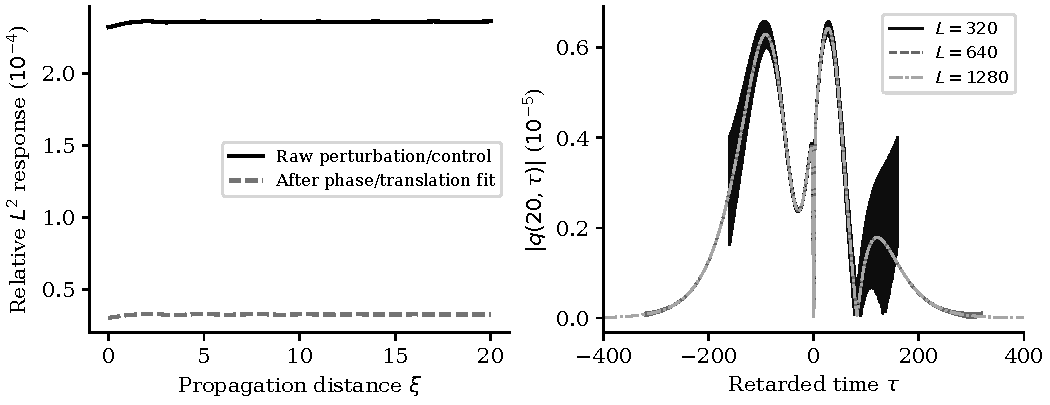
\includegraphics[width=\linewidth]{figures/shape-and-drift.pdf}\caption{Raw versus fitted response and the final signed-response magnitude. Nearly equal scalar shape norms can hide substantially different radiation fields; the convergence tests compare the complex fields themselves.}\end{figure}

\subsection{Residuals, invariants, and resources}

The largest initial/final discarded-RHS ratio in the accepted-spacing, small-step cases is $9.29\times10^{-12}$. This is an instantaneous resolution diagnostic, not a time-integrated error bound. The following invariant maxima cover both control and odd trajectories; energy and momentum are the continuum functionals rather than assumed exact discrete invariants.

\begin{center}
\small
\begin{tabular}{lrrr}
\toprule
$L$ & Action drift & Energy drift & Momentum drift \\
\midrule
160 & $8.66\times10^{-13}$ & $2.72\times10^{-12}$ & $6.74\times10^{-11}$ \\
640 & $6.29\times10^{-13}$ & $1.98\times10^{-12}$ & $6.74\times10^{-11}$ \\
1280 & $7.30\times10^{-13}$ & $2.30\times10^{-12}$ & $6.73\times10^{-11}$ \\
\bottomrule
\end{tabular}
\end{center}


The five new full-horizon cases used 809.2 process-wall seconds in total, with peak recorded process RSS 177.9 MiB. Some cases ran concurrently, so these durations are not elapsed session time. The benchmark used less than one second. Every saved field was finite. The existing large-window sech initial guess emitted one benign cosh-overflow warning in its vanishing tails; it did not produce nonfinite profiles or trajectories.

\subsection{Recommendation and accuracy limits}

\textbf{Go for the next small initial-data simulator, after review, using this periodic equation and per-case qualification.} The reference passes analytic controls, independent residual checks, fourth-order step convergence, and independent grid convergence. No change to the equation or propagator was needed. The added diagnostics separate symmetry drift and identify the domain failure mechanism.

For an illustrative one-percent signed weak-response agreement target, the sampled horizons of the smaller windows are $\xi\leq 5$ for $L=160$, $\xi\leq 10$ for $L=320$, and $\xi\leq 20$ for $L=640$, each assessed against the next doubled domain. These are measured sample-wise agreements for this perturbation, not rigorous error bars or universal domain choices.

The final $640/1280$ common-window shape discrepancy is $1.75\times10^{-7}$, or 0.538\% of this weak shape response. A full-domain initial-data simulator must preserve phase, translation, and radiation and expose numerical-resolution checks. New focusing, modulation, and bandwidth ranges need their own convergence evidence.

\textbf{No-go for a large training corpus or FNO training now.} The original $L=160$, $\xi=20$ setup is not qualified as an isolated weak-radiation reference. The entire legacy profile library is not qualified either. The next stage should implement a small plug-and-play simulator with a finite, explicitly tested input range; dataset generation and learning require a later decision. Short persistence does not establish soliton discovery or stability.


\clearpage
\section{Reproducibility}
The checked snapshot is \path{stage1/source/}; additive modules are installed
in the original project's \texttt{dysthe-core} and \texttt{dysthe-experiments}
repositories. The installation manifest lists all nine added files and hashes.
Initial provenance, effective
configurations, SHA-256 hashes, environment versions, timings, and sampled
complex fields accompany the results. Existing unrelated changes and
historical arrays are preserved.

Full commands are recorded in \path{stage1/README.md}. From the task root,
use the two snapshot source directories and the existing project's
\path{dysthe-learning/src} on \texttt{PYTHONPATH}. Run
\texttt{pytest --import-mode=importlib -p no:cacheprovider}, followed by
these experiment modules (\texttt{project} denotes the verified project):
\begin{verbatim}
python3 -m dysthe_experiments.reference_controls \
  --profiles "$project/results/nonlinear" \
  --output stage1/results/analytic-checks.json
python3 -m dysthe_experiments.reference_stage_one \
  --profile "$profile" --output stage1/results/benchmark --benchmark
python3 -m dysthe_experiments.reference_stage_one \
  --profile "$profile" --output stage1/results/campaign
python3 -m dysthe_experiments.reference_stage_one \
  --profile "$profile" --extended-domain --output stage1/results/extended
python3 -m dysthe_experiments.reference_analysis \
  --historical "$actualruns" --campaign stage1/results/campaign \
  --extended stage1/results/extended --output stage1/results/analysis
python3 stage1/make_report_results.py
\end{verbatim}
The initial-data simulator needs new per-family qualification, especially
for focusing and radiation. This stage contains no training dataset, FNO
training, paid compute, or HPC submission. Its finite periodic evidence
also supplies no Euler-equation or experimental validation.

\begin{thebibliography}{9}
\bibitem{fedele2012}
F. Fedele and D. Dutykh,
\emph{Hamiltonian description and traveling waves of the spatial Dysthe
 equations}, arXiv:1110.3605v3, 12 April 2012.
\url{https://arxiv.org/html/1110.3605v3}.
\end{thebibliography}
\end{document}
